\section{Background}
Energy consumption is ever increasing and our current electrical grid is outdated, as it is unable to handle the more dynamic production and consumption of power we have today.
There is also an increasing generation of renewable energy (e.g. wind and solar), but optimal use of this is limited by our current electrical grid.
As it is now, renewable sources are often shut down if they are producing more than can be consumed.
On the other hand, during periods with little renewable power, more expensive and environmentally unsafe sources are used.

Additionally most net suppliers only support very simple tariffs with one fixed price, or a single division of prices, throughout the day.

The statements above have led to an increased focus on energy usage, with optimizations of the electrical grid as a high priority, which is why by 2022 all\footnote{80\% by 2020} electrical meters in EU member countries must be replace by \textit{smart meters} \cite{smart_meter_survey, directive_2009_72_EC}.
An expansion of the electrical grid, as it is extended to connect more EU member countries, along with the addition of smart meters -- enabling home owners to supply themselves and others, will form a \textit{smart grid}.

\subsection{Smart Grid and Smart Meters}
A smart grid is an electrical grid supported by a net, allowing two-way communication, whereas earlier it was only one-way.
This allows for much more dynamic power supply and consumption, as suppliers will know more about their consumers, and consumers will have more options in regards to their consumption.

The outline of a smart grid can be seen in \cref{fig:background:smartgrid}.
This consists of three main actors:
Power suppliers such as Windmills, solar panels, traditional power plants and external suppliers.
A net supplier such as a Datahub \footnote{Danish term from \cite{LOV_nr_575_af_18-06-2012}} and smart meters.
End consumers such as smart homes/buildings.

A smart grid serves several purposes, such as allowing for/enabling \cite{smartgrid_gov, directive_2009_72_EC}:
\begin{itemize}
	\item prices to be based on supply and demand.
	\item prices to be based on type of power available.
	\item connecting electrical grids across Europe.
	\item easier changing of energy supplier.
	\item more detailed monitoring of power consumption.
	\item adjusting power consumption based on available power/prices.
	\item consumers to also be suppliers to the smart grid (windmills, solar panels, etc.).
	\item use of smart appliances (see \cref{background:smart_appliances}).
\end{itemize}

\begin{figure}
	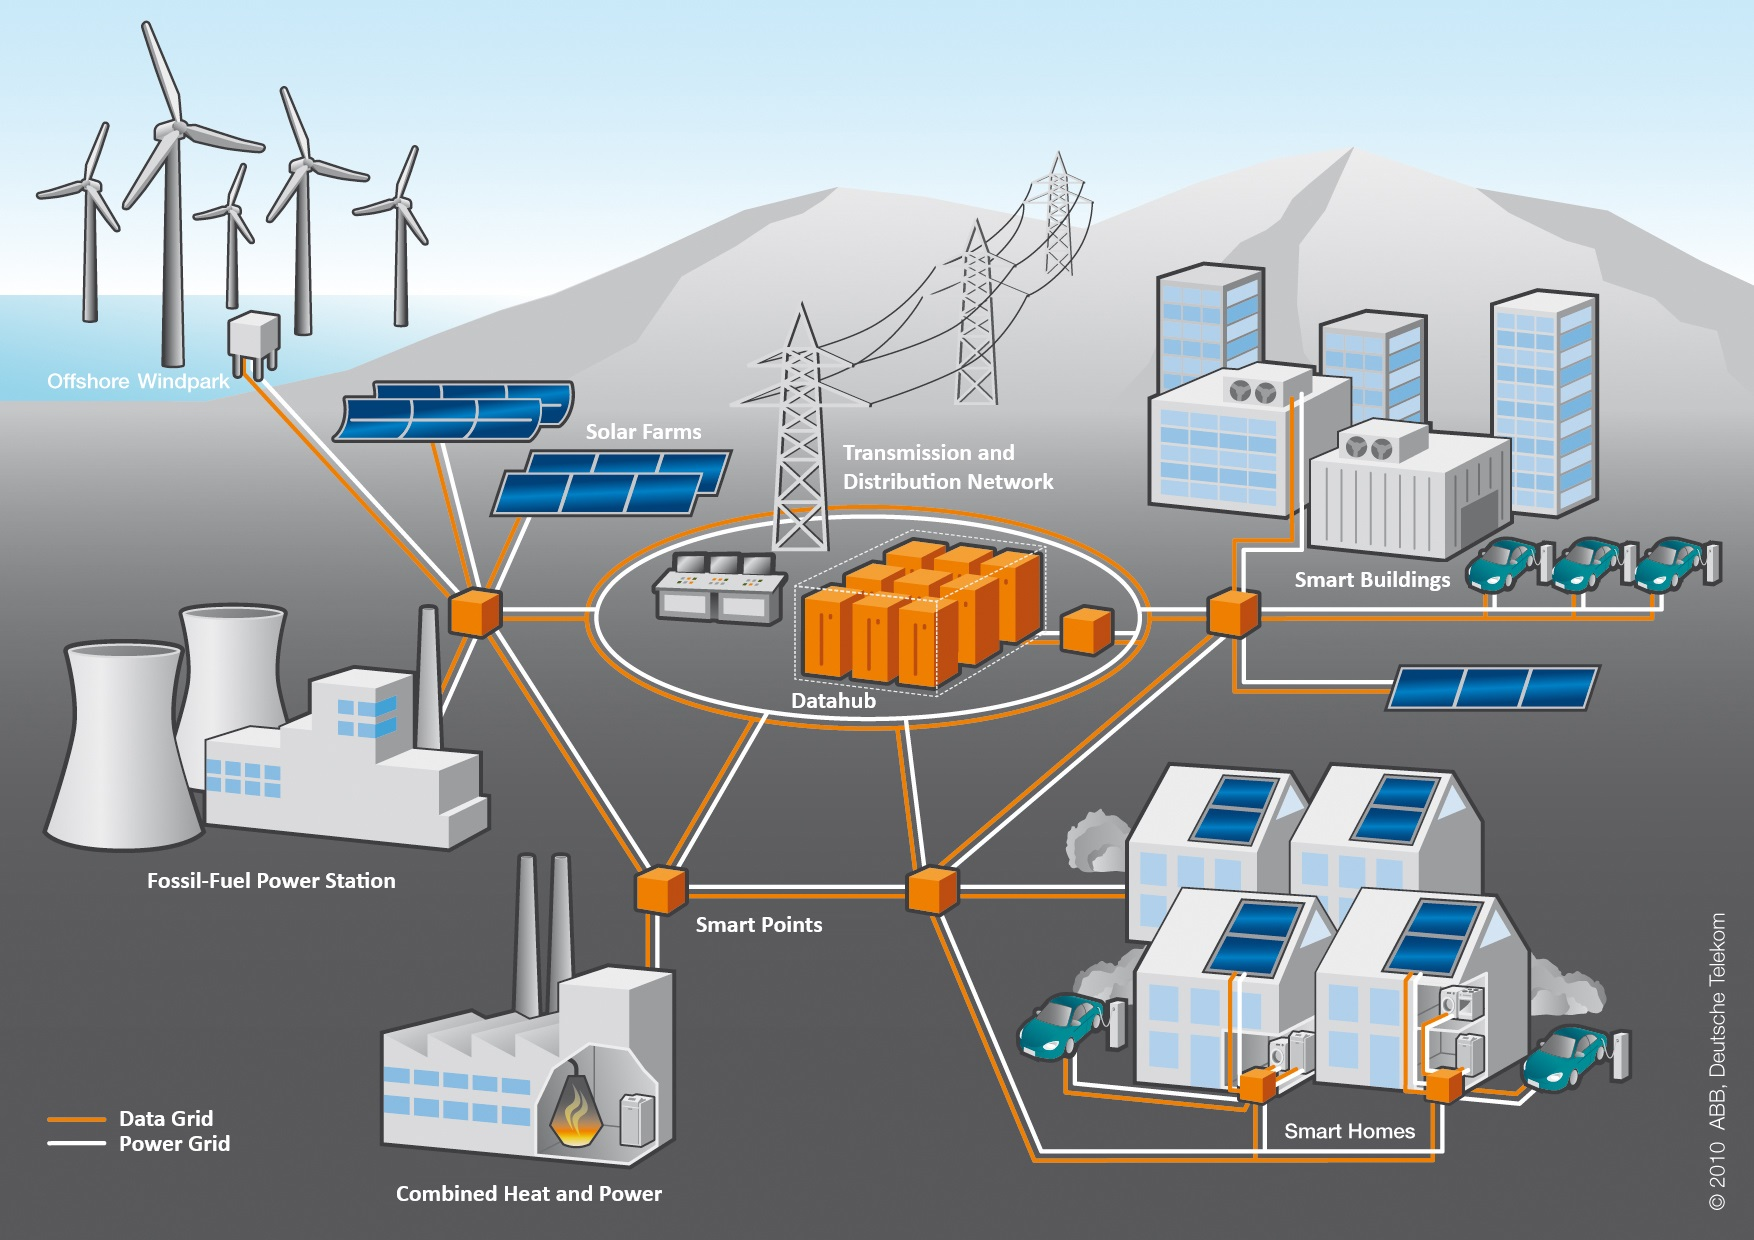
\includegraphics[width=\textwidth]{figures/SmartGrid_Ueberblick_ohneLegende.jpg}
	\caption{Smart grid outline\protect\footnotemark}
	\label{fig:background:smartgrid}
\end{figure}
\footnotetext{\url{https://www.telekom.com/medien/bild-ton-und-infografiken/infografiken/155030}}

\subsubsection{Smart appliances}
\label{background:smart_appliances}
Smart appliances\cite{smart_appliances} are ordinary appliances, such as air conditioners, refridgerators, or dishwashers.
What makes them smart is the fact that the times or periods in which they are turned on are highly configurable, so that they can match changing power prices.
This can be done manually, by the user looking at current pricing and setting a timer when to turn on.
However, some smart appliances can also by themselves look up prices and choose appropriate times to turn on.

\subsection{Problems}
In regards to enabling an EU-wide smart grid, there are bound to be problems, as this is an immense project.
The roll-out will not be the same in every nation, as each nation has its own infrastructure and legal constraints.
Additionally they differ in which parts of their electrical grids are privately and publicly owner.
However, some shared problems still exist, such as privacy, conflicts of interest, and attack vulnerabilities \cite{offswitch, smart_meter_survey, security_economics}.

\subsubsection{Different architectures}
\bruno{\#2}
\begin{itemize}
	\item Italy - regulated monopoly (supplier and distibutor is the same?)
	\item Germany - Free market for both distributor (people buy smart meter device/maintenance) and supplier
	\item UK - Centralized government-licensed monopoly
	\item DK - Centralized through 60 government-regulated distributors, datahub contains/controls all power usage data
\end{itemize}

\subsubsection{Privacy}
With the adaptation of smart meters it will be possible to collect power usage data more often.
This is possible as it can be done remotely, whereas earlier a display would have to be read on the physical electrical meter.
It also makes sense to have more readings, as tariffs will vary more, and therefore more measurements are needed to match prices during tariff-determined periods.
\mikkel{\#3: The last point here seems to be taken out of thin air.
How do we know that they will vary more?}

This possibility of finer granularity meter readings can be exploited in several ways and by different actors.
The supplier would like this information in order to better tailor prices for a certain customer, thus limiting competition as their competitors do not possess this information.
If the power usage data was obtained by an electronics vendor, they could use it to target certain advertisements, based on what devices they detect (or don't detect) through the power usage.
Anyone with malicious intent could use the power data to determine who, if anyone, is home (e.g. burglars).
Finally, the government could use this data to surveil the public.

Some important issues with smart meters and their measurements are therefore:
\begin{itemize}
	\item Who owns the data?
	\item Who should be able to access the data?
	\item With which granularity should supplier/government/user be able to access the data?
	\item How do we ensure that only the correct people have access to the smart meter and its data?
\end{itemize}

\subsubsection{Conflict of interest}
The various actors involved with smart grids have different interests and potential gains.
Governments generally want lower consumption for environmental reasons.
They especially want consumption down during peak hours, in order to avoid the usage of environmentally unfriendly energy sources.
Depending on tariffs, suppliers might also want power consumption down during peak hours if they cannot provide enough, from their perspective, cheap energy.
However, suppliers generally want high consumption, so that they can sell more power and thus make more money.
Consumers want to use power as needed, but at lower costs.

These interests exemplify considerations by actors in a smart grid system.
Naturally there could be more such as consumers and suppliers having environmental considerations or governments seeking to increase productivity on a national level with lower regards for the environment.

The above relations spark several conflicts of interest:
\begin{itemize}
	\item Should governments be able to control user power consumption? If so, how?\footnote{E.g. carbon rationing in the UK \cite{security_economics}}
	\item Should others than the user be able to turn off the power? (See \cite{offswitch}\bruno{Ref to related work, look \#4}) If so,
	\begin{itemize}
		\item who should be able to use this?
		\item how should it work? (With abuse in mind.)
	\end{itemize}
	\item How, and by whom, should smart appliances be managed?
\end{itemize}

\subsubsection{Vulnerabilities}
In the current system consumeres are already tampering  with their mechanical electrical meters.
Turning these mechanical meters into smart meters will possibly remove attacks, but will definitely open up for new attacks.
Switching to smart meters introduces a new branch of attacks; digital attacks.
These include attacks that are general to any publicly exposed unit, or any unit that sends data over public networks.
